\chapter{Zadatak 1}

\textbf{1.} U ovom dijelu zadatka je potrebno identificirati parametre stvarnog sistema opisanog funkcijom G(s) u koju su uvrštene vrijednosti a=2 i b=2 (u svrhu proračuna). Funkcija G(s) zadana je kao:

	\[ G(s)=\frac{3.2}{120s^4+417s^3+415.5s^2+127.5s+9} \]


Identifikaciju je potrebno uraditi analizom odziva na jediničnu pobudnu funkciju te aproksimirati dati sistem sistemom prvog reda sa čistim transportnim kašnjenjem $G_{ident} (s)$.
	\[G_{ident} (s)=\frac{k_{ob}}{T_{ob} s+1} e^{-\tau_{ob} s} \]


\begin{figure} [H]
  \centering
  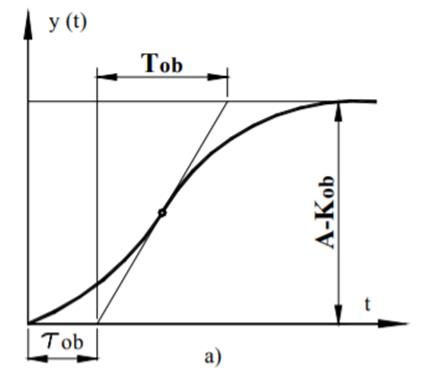
\includegraphics[width=0.6\textwidth]{z1_1}
  \caption{Odziv na jediničnu pobudnu funkciju nekog sistema}
  \label{fig:z1_1}
\end{figure}



Na osnovu odziva na jediničnu pobudnu funkciju koji je skiciran na prethodnoj slici (slika \ref{fig:z1_1}), određuju se parametri prenosne funkcije $G_{ident} (s)$ na sljedeći način:
	\[k_{ob}=\frac{Y(\infty)-Y(0)}{A} \]


gdje su: 
\begin{itemize}
    \item $Y(\infty)$ - veličina odziva u novom stacionarnom stanju
    \item $Y(0)$ - veličina odziva u starom stacionarnom stanju
    \item A - amplituda ispitne funkcije (u ovom slučaju jedinična funkcija amplitude A=1.
\end{itemize}
	  
Preostala dva parametra $\tau_{ob}$ i $T_{ob}$ se mogu odrediti na sljedeći način. Pronađemo prevojnu tačku dobivenog odziva na jediničnu pobudnu funkciju. Nakon toga povučemo tangentu u toj prevojnoj tački (slika \ref{fig:z1_1}) te odredimo tačke presjeka sa starim i novim stacionarnim stanjem. Nakon toga, kao što je to prikazano na slici (slika \ref{fig:z1_1}) možemo odrediti ova dva parametra.

Provedbom opisanog postupka u MATLAB-u dobivena je sljedeća prenosna funkcija:
	\[G_{ident} (s)=\frac{0.3555}{16.66s+1} e^{-2.67s} \]

Sada će biti prikazan step odziv (slika \ref{fig:z1_2}), impulsni odziv (slika \ref{fig:z1_3}), Bode dijagrami (slika \ref{fig:z1_4}) te raspored nula i polova (slika \ref{fig:z1_5}) stvarnog i aproksimiranog sistema.

\begin{figure} [H]
  \centering
  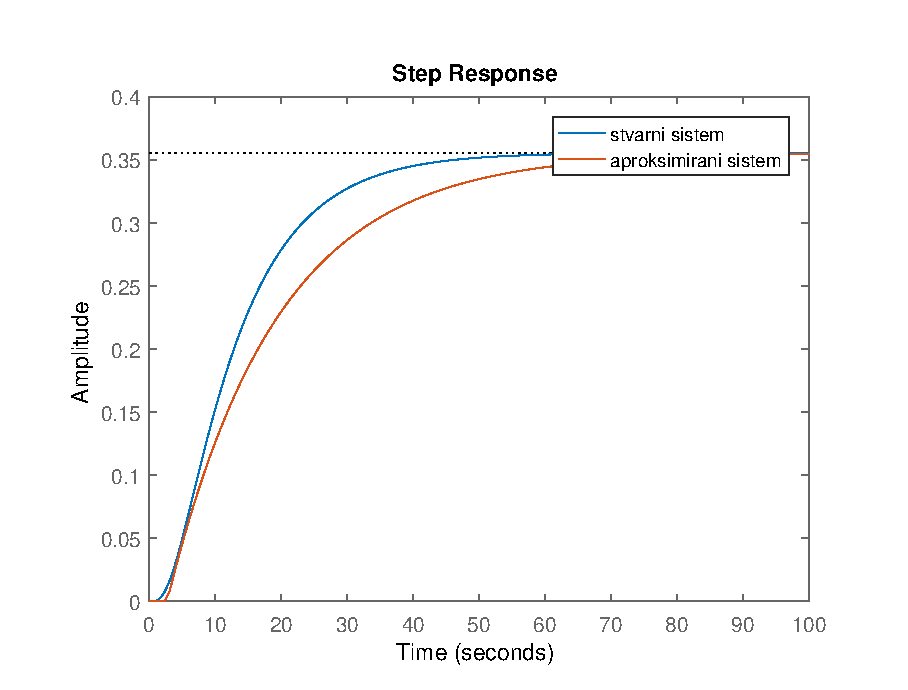
\includegraphics[width=0.9\textwidth]{z1_2}
  \caption{Identifikacija: odzivi sistema na step}
  \label{fig:z1_2}
\end{figure}

\begin{figure} [H]
  \centering
  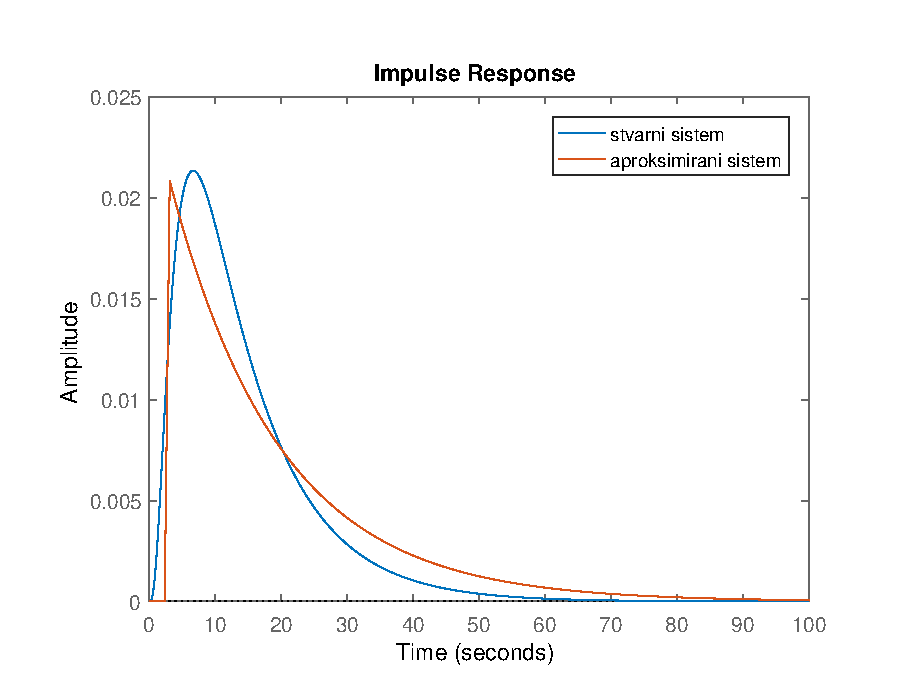
\includegraphics[width=0.9\textwidth]{z1_3}
  \caption{Identifikacija: impulsni odzivi sistema}
  \label{fig:z1_3}
\end{figure}

\begin{figure} [H]
  \centering
  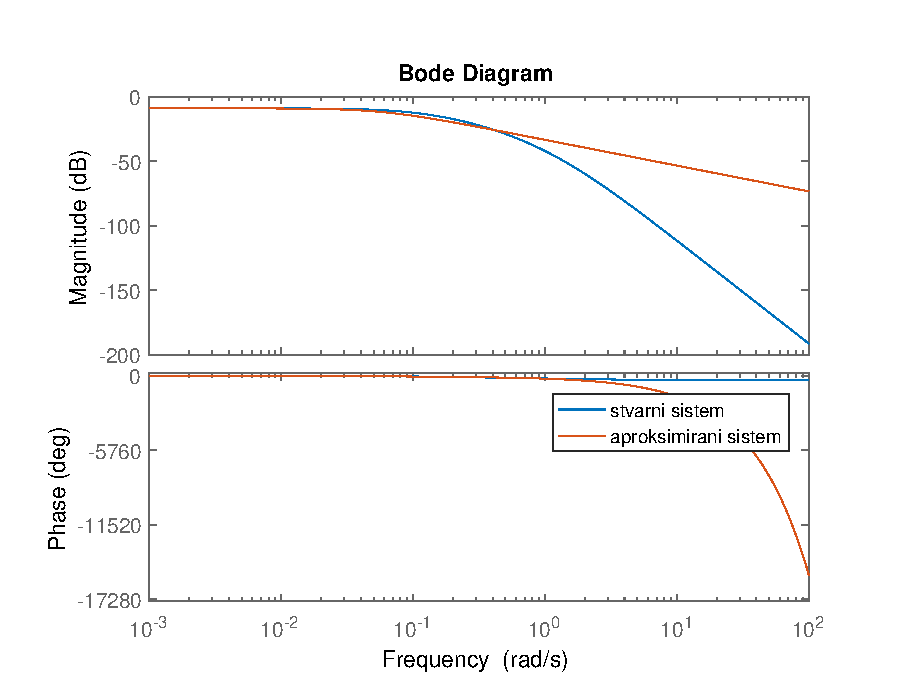
\includegraphics[width=0.9\textwidth]{z1_4}
  \caption{Identifikacija: Bode dijagrami sistema}
  \label{fig:z1_4}
\end{figure}
 

Možemo primijetiti da sistem prvog reda sa čistim transportnim kašnjenjem ima eksponencijalno opadajuću fazu (zbog logaritamske razmjere), tj. ima linearnu fazu zbog elementa transportnog kašnjenja. Što se tiče amplitudne karakteristike, i jedan i drugi sistem se ponašaju kao niskopropusni filteri, jedina je razlika što zbog reda sistema nakon prelomne frekvencije stvarni sistema ima jače slabljenje viših frekvencija zbog većeg reda sistema.
 
 \begin{figure} [H]
  \centering
  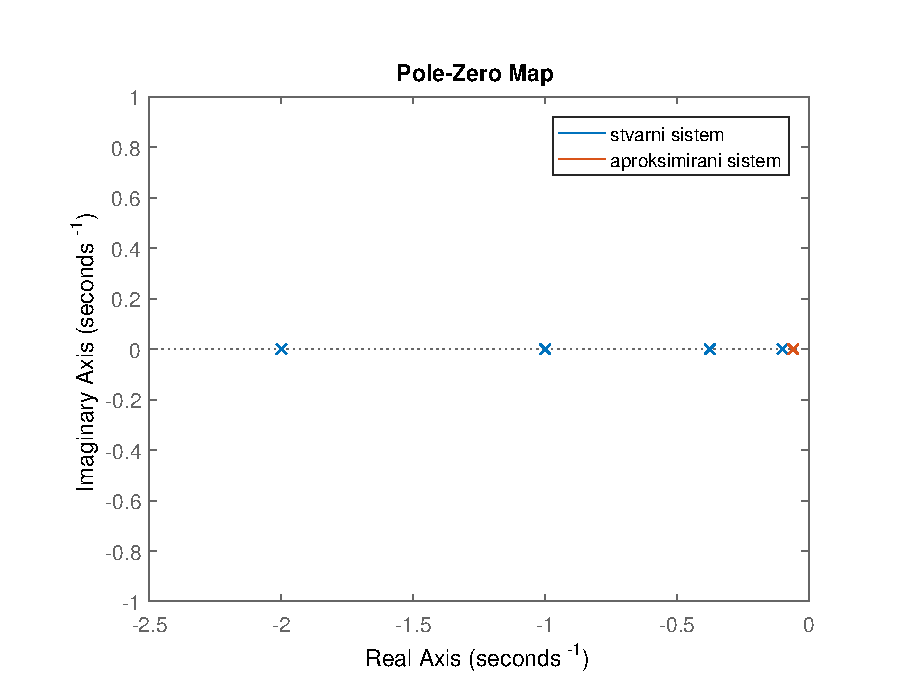
\includegraphics[width=0.9\textwidth]{z1_5}
  \caption{Identifikacija: polovi i nule sistema}
  \label{fig:z1_5}
\end{figure}
 
Stvarni sistem je sistem 4. reda koji ima 4 pola. Dva konjugovano kompleksna pola su dominantna, ali zbog blizine nule njihov utjecaj slabi. Pol sistema prvog reda sa transportnim kašnjenjem je postavljen tako da aproksimira dinamiku sistema 4. reda, a postavljen je blizu dominantnog pola stvarnog sistema 4. reda. Ostali polovi imaju slabiji utjecaj na odziv sistema 4. reda pa je ova aproksimacija sistemom prvog reda sa čistim transportnim kašnjenjem dobra aproksimacija.

\textbf{2.} U ovom dijelu će biti pokazani regulacioni krugovi napravljeni u Simulink-u za potrebe testiranja PID regulatora za aproksimirani i stvarni sistem (slika \ref{fig:z1_6}).
 
  \begin{figure} [H]
  \centering
  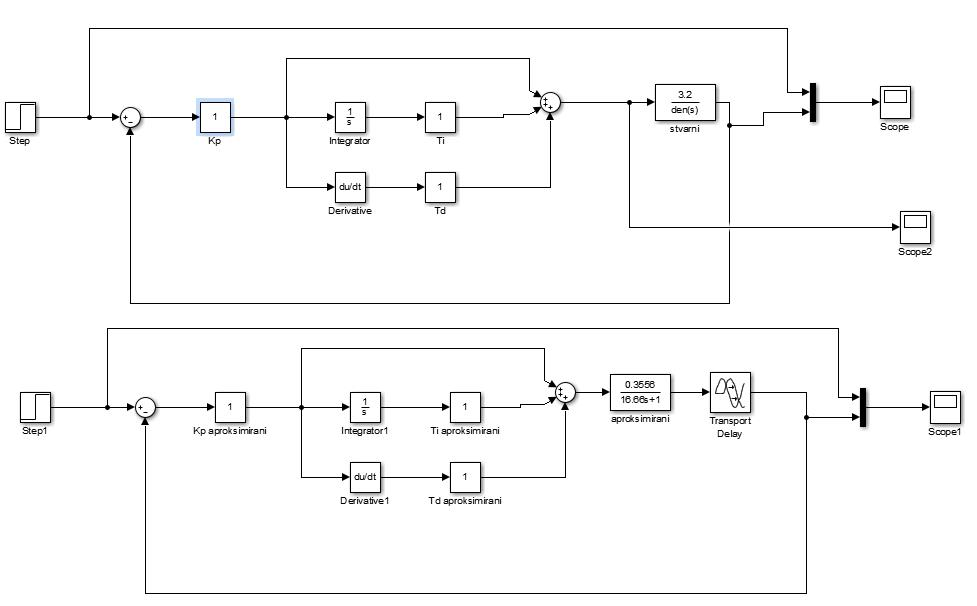
\includegraphics[width=0.9\textwidth]{z1_6}
  \caption{Regulacioni krugovi u Simulink-u u kojima je moguće varirati parametre PID regulatora za stvarni i aproksimirani sistem}
  \label{fig:z1_6}
\end{figure}
 
 \textbf{3.} 	Povećanjem pojačanja $K_p$ postižemo brži odziv (slika \ref{fig:z1_7}). Također, u tom slučaju dolazi do smanjenja greške u stacionarnom stanju koju ipak nije moguće otkloniti kada koristimo samo P regulator jer kada bi greška postala jednaka nuli, tada ne bi bilo nikakvog djelovanja na sistem. To znači da će greška u stacionarnom stanju kod P regulatora uvijek postojati. Također, povećanjem pojačanja $K_p$ možemo učiniti sistem nestabilnim.
 
 \begin{figure} [H]
  \centering
  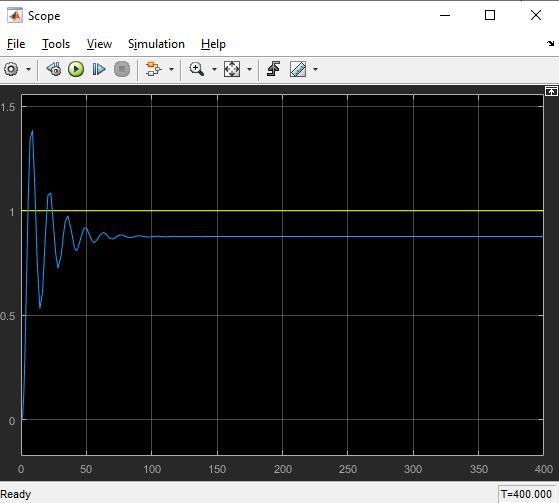
\includegraphics[width=0.7\textwidth]{z1_7}
  \caption{Odziv stvarnog sistema za $K_p=20$}
  \label{fig:z1_7}
\end{figure}


Dodavanjem djelovanja integralne komponente (slika \ref{fig:z1_8}) postižemo eliminisanje greške u stacionarnom stanju. Međutim, dolazi do većeg preskoka i povećanja vremena smirenja jer je došlo do oscilacija. Vrijeme porasta se smanjuje jer će integralna komponenta na početku generisati dodatno pojačanje u sistem sumiranjem pozitivne greške (greška kada se oduzmu zadana i trenutna vrijednost koja kreće iz nule).

\begin{figure} [H]
  \centering
  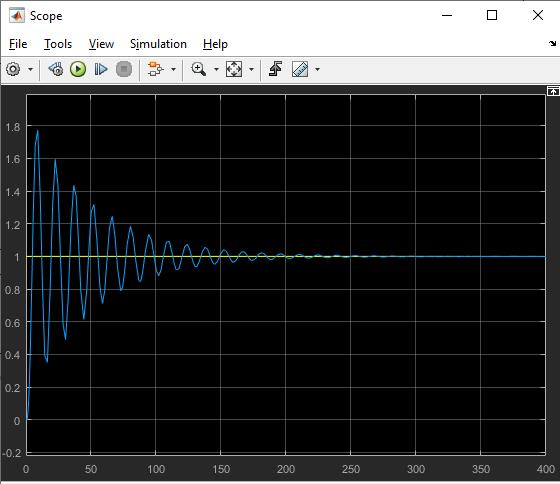
\includegraphics[width=0.8\textwidth]{z1_8}
  \caption{Odziv stvarnog sistema za $K_p=20$, $T_i=10$}
  \label{fig:z1_8}
\end{figure}

Sada je potrebno dovesti sistem u nestabilno stanje, a zatim primijeniti D komponentu PID regulatora. Izabrano je $T_i=2$ jer je tada sistem nestabilan. Dodavanjem D komponente (slika \ref{fig:z1_9}) PID regulatora sistem ponovo postaje stabilan. Dakle, P i I komponentu možemo još više pojačati za razliku od PI regulatora. Također, D komponetna povećava rezerve stabilnosti tako da je moguće sistem ustabiliti ukoliko je bio nestabilan (što je ovdje slučaj). D komponenta također smanjuje prvi preskok jer kaže kontroleru ako počne brzo da raste da uspori odziv, i obrnuto. Također, D komponenta smanjuje oscilacije u sistemu pa zbog toga smanjuje vrijeme smirenja.

\begin{figure} [H]
  \centering
  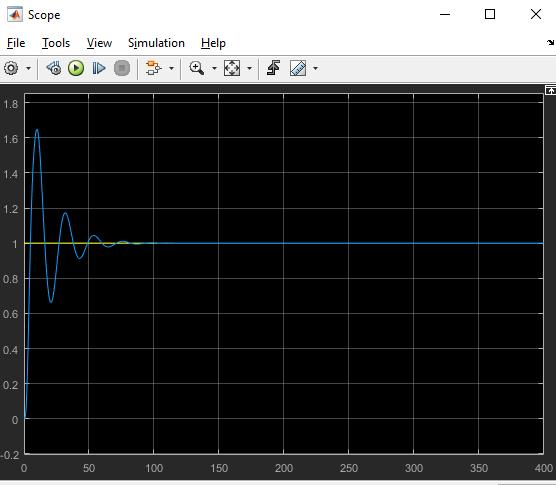
\includegraphics[width=0.8\textwidth]{z1_9}
  \caption{Odziv stvarnog sistema za $K_p=20$, $T_i=2$, $T_d=5$}
  \label{fig:z1_9}
\end{figure}

\textbf{4.} Da bismo izračunali kritično pojačanje $k_{rkrit}$ analitički, potrebno je da riješimo jednačinu:
	\[1+KG(s)=0	\]

Povećavamo pojačanje od nule ka većim vrijednostima sve dok ne dobijemo da je jedno ili više rješenja ove jednačine čisto imaginarno, a ostala rješenja sa realnim dijelom manjim od nule. Tada je sistem na granici stabilnosti. Pojačanje za koje dobijemo navedene rezultate je kritično pojačanje $k_krit$.

Kritično pojačanje je moguće odrediti na više načina primjenom MATLAB-ovih toolbox-a. Pa tako pored već navedenog načina, moguće je odrediti kritično pojačanje na sljedeće načine:
	\begin{itemize}
	    \item korištenjem sisotool toolbox-a te variranjem pojačanja K dok neki od polova u zatvorenom ne dođe na granicu stabilnosti
	    \item crtanjem Nyquist-ove karakteristike, pri tome varirajući pojačanje K dok ne dobijemo da karakteristika prolazi kroz kritičnu tačku (-1,j0)
	    \item korištenjem Bode-ovih dijagrama tako što gledamo rezerve stabilnosti, tj određujemo za koju vrijednost pojačanja K će rezerva stabilnosti po pojačanju biti jednaka nuli ili rezerva stabilnosti po fazi biti nula stepeni.
	\end{itemize}
	
Korištena je metoda u kojoj pojačanje variarmo u sisotool toolbox-u te određujemo kritično pojačanje (slika \ref{fig:z1_10}).

\begin{figure} [H]
  \centering
  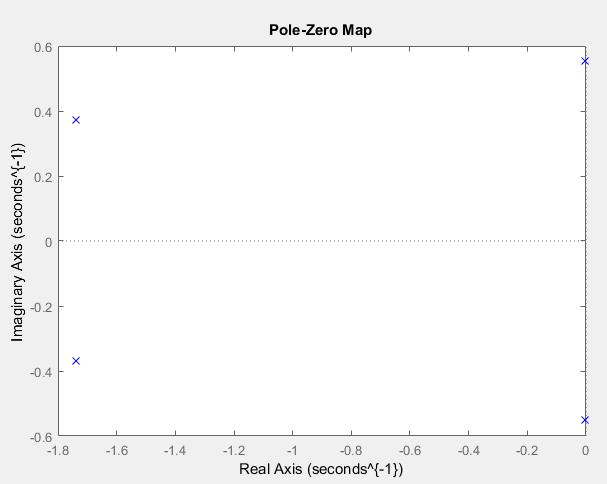
\includegraphics[width=0.8\textwidth]{z1_10}
  \caption{GMK karakteristika stvarnog sistema sa polovima u zatvorenom na imaginarnoj osi, pri čemu je dobiveno pojačanje od $k_{krit}=33.382$ (slika u donjem desnom uglu)}
  \label{fig:z1_10}
\end{figure}

\begin{figure} [H]
  \centering
  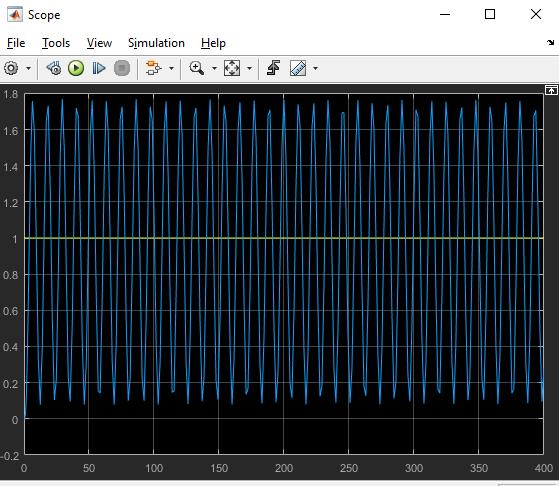
\includegraphics[width=0.8\textwidth]{z1_11}
  \caption{Simulirani odziv na step za dobiveno kritično pojačanje $k_{krit}=33.382$}
  \label{fig:z1_11}
\end{figure}

Simuliranjem odziva na step za dobiveno kritično pojačanje $k_{krit}=33.382$, dobijamo stabilne oscilacije (slika \ref{fig:z1_11}) na izlazu perioda $T_{krit}=11.384s$.

\textbf{5.}	Potrebno je podesiti parametre za tri vrste regulacije (P, PI, PID) na osnovu Ziegler-Nichols metode za stvarni sistem. Način podešavanja na osnovu pronađenih vrijednosti $k_{krit}=33.382$ i $T_{krit}=11.384s$ je dat u tabeli prikazanoj slikom \ref{fig:z1_12}
 
\begin{figure} [H]
  \centering
  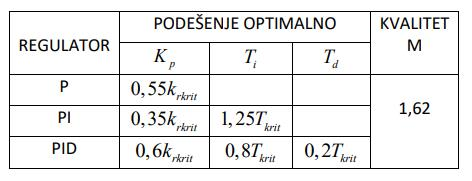
\includegraphics[width=0.5\textwidth]{z1_12}
  \caption{Tabela podešavanja parametara P, PI, PID regulatora Ziegler-Nichols metodom za stvarni sistem}
  \label{fig:z1_12}
\end{figure}

Dobiveni rezultati:

\textbf{P regulator: $K_p=18.36$} (slika \ref{fig:z1_13})

\begin{figure} [H]
  \centering
  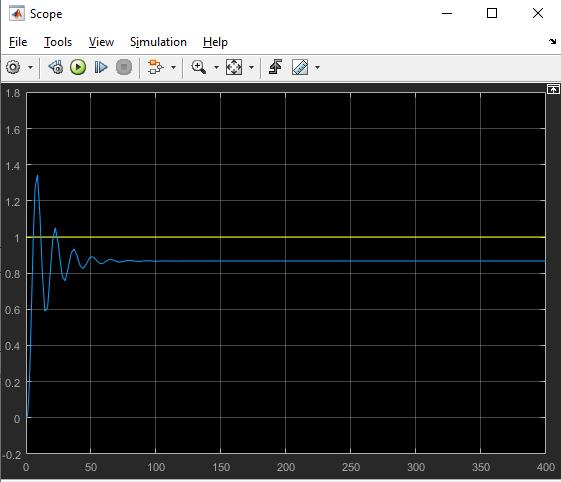
\includegraphics[width=0.8\textwidth]{z1_13}
  \caption{Odziv zatvorenog sistema sa P regulatorom dobivenim Ziegler-Nichols metodom}
  \label{fig:z1_13}
\end{figure}

\textbf{PI regulator: $K_p=11.68$, $T_i=14.23$} (slika \ref{fig:z1_14})

\begin{figure} [H]
  \centering
  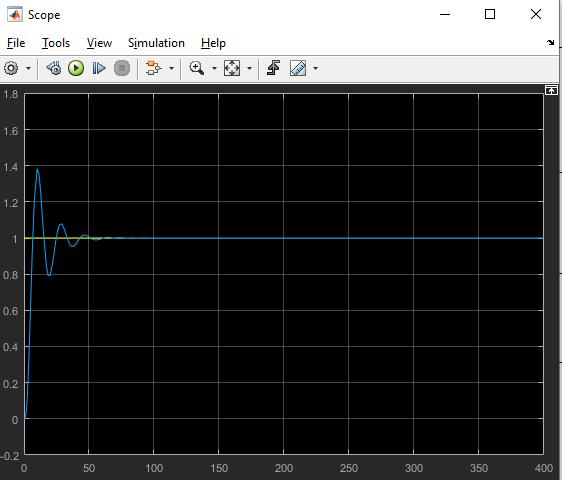
\includegraphics[width=0.8\textwidth]{z1_14}
  \caption{Odziv zatvorenog sistema sa PI regulatorom dobivenim Ziegler-Nichols metodom}
  \label{fig:z1_14}
\end{figure} 

\textbf{PID regulator: $K_p=20.0292$, $T_i=9.1072$, $T_d=2.2768$} (slika \ref{fig:z1_15})

\begin{figure} [H]
  \centering
  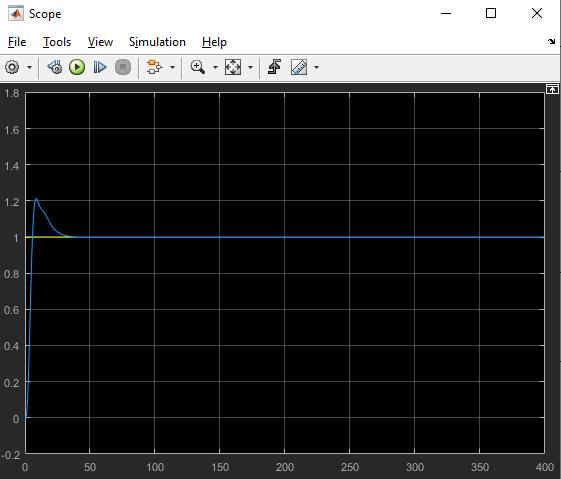
\includegraphics[width=0.7\textwidth]{z1_15}
  \caption{Odziv zatvorenog sistema sa PID regulatorom dobivenim Ziegler-Nichols metodom}
  \label{fig:z1_15}
\end{figure} 

\textbf{6.} 	Potrebno je podesiti parametre za tri vrste regulacije (P, PI, PID) na osnovu Ziegler-Nichols metode za aproksimirani sistem. Način podešavanja je dat u tabeli:
 
\begin{figure} [H]
  \centering
  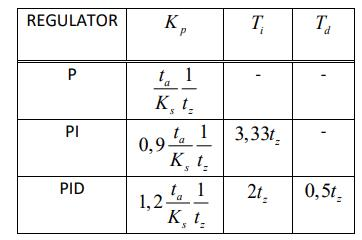
\includegraphics[width=0.5\textwidth]{z1_16}
  \caption{Tabela podešavanja parametara P, PI, PID regulatora Ziegler-Nichols metodom za aproksimirani sistem}
  \label{fig:z1_16}
\end{figure}

Vrijednosti koje se nalaze u tabeli se mogu vidjeti na sljedećem grafiku (\ref{fig:z1_17}):
 
 \begin{figure} [H]
  \centering
  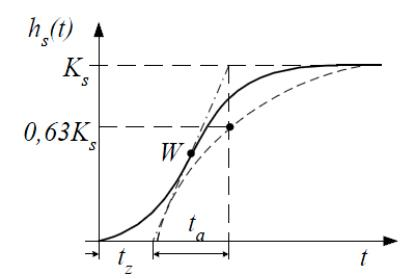
\includegraphics[width=0.5\textwidth]{z1_17}
  \caption{Step odziv na osnovu kojeg dobivamo aproksimirani sistem}
  \label{fig:z1_17}
\end{figure}

Kako je prenosna funkcija aproksimiranog sistema (izračunato pod a)) data kao:
	\[G_{ident} (s)=\frac{0.3555}{16.66s+1} e^{-2.67s} \]

Tako je: $t_z=2.67$, $t_a=16.66$, $K_s=0.3555$. Na osnovu ovih parametara i tabele iz koje se određuju parametri P, PI i PID regulatora su dobiveni sljedeći rezultati:

\textbf{P regulator: $K_p=17.5519$} (slika \ref{fig:z1_18})
 
\begin{figure} [H]
  \centering
  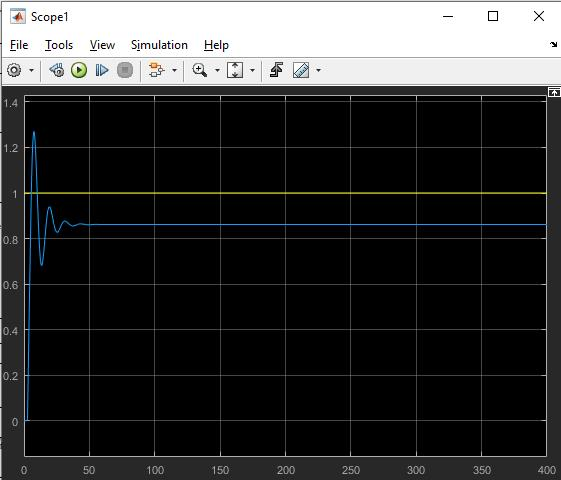
\includegraphics[width=0.8\textwidth]{z1_18}
  \caption{Odziv zatvorenog sistema sa P regulatorom dobivenim Ziegler-Nichols metodom (2)}
  \label{fig:z1_18}
\end{figure} 

\textbf{PI regulator: $K_p=15.7967$, $T_i=8.8911$} (slika \ref{fig:z1_19})
 
\begin{figure} [H]
  \centering
  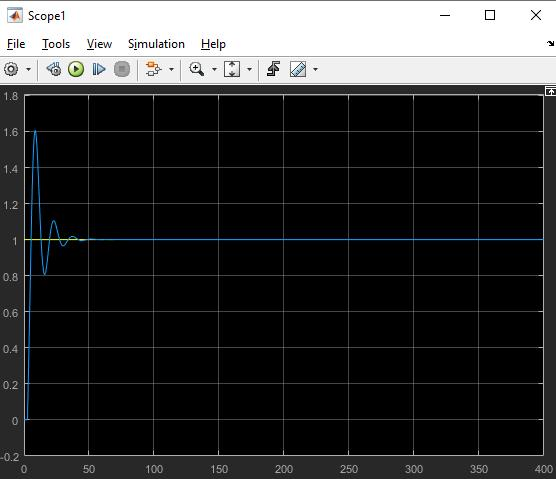
\includegraphics[width=0.75\textwidth]{z1_19}
  \caption{Odziv zatvorenog sistema sa PI regulatorom dobivenim Ziegler-Nichols metodom (2)}
  \label{fig:z1_19}
\end{figure} 

\textbf{PID regulator: $K_p=21.0623$, $T_i=5.34$, $T_d=1.335$} (slika \ref{fig:z1_20})

\begin{figure} [H]
  \centering
  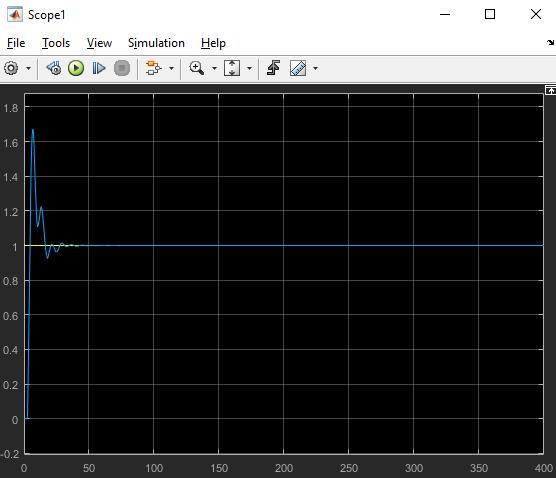
\includegraphics[width=0.8\textwidth]{z1_20}
  \caption{Odziv zatvorenog sistema sa PID regulatorom dobivenim Ziegler-Nichols metodom (2)}
  \label{fig:z1_20}
\end{figure}  

\textbf{7.} Potrebno je podesiti parametre za tri vrste regulacije (P, PI, PID) na osnovu Cohen-Coon metode za aproksimirani sistem. Način podešavanja je dat u tabeli:
 
\begin{figure} [H]
  \centering
  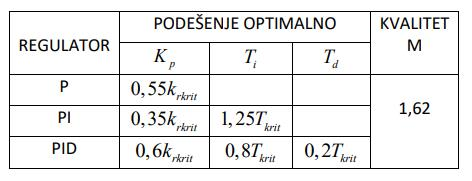
\includegraphics[width=0.6\textwidth]{z1_12}
  \caption{Tabela podešavanja parametara P, PI, PID regulatora Cohen-Coon metodom za aproksimirani sistem}
  \label{fig:z1_12}
\end{figure}
 
Parametri potrebni za izračunavanje parametara P, PI i PID regulatora su dobiveni u stavci pod 5) i iznose: $t_z=2.67$, $t_a=16.66$, $K_s=0.3555$. Na osnovu ovih parametara dobiveni su sljedeći rezultati:

\textbf{P regulator: $K_p=18.4895$} (slika \ref{fig:z1_22})
 
 \begin{figure} [H]
  \centering
  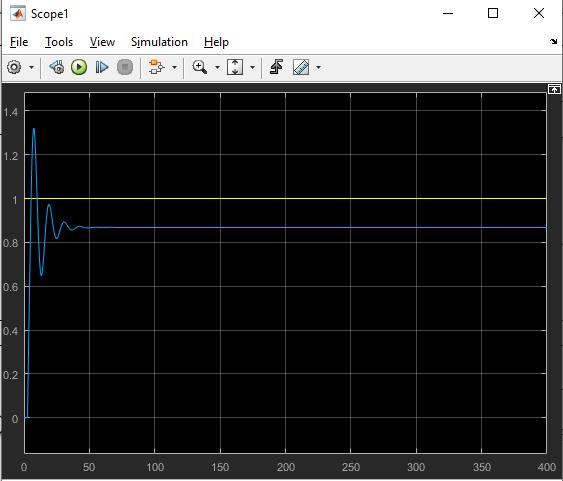
\includegraphics[width=0.8\textwidth]{z1_22}
  \caption{Odziv zatvorenog sistema sa P regulatorom dobivenim Cohen-Coon metodom}
  \label{fig:z1_22}
\end{figure} 

\textbf{PI regulator: $K_p=16.0311$, $T_i=3.8745$} (slika 2\ref{fig:z1_23})
 
\begin{figure} [H]
  \centering
  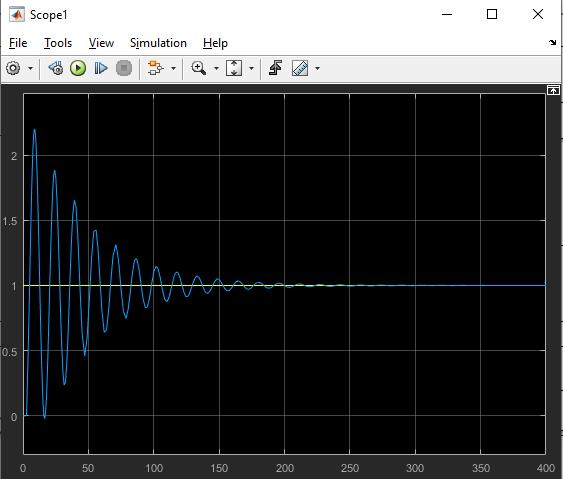
\includegraphics[width=0.75\textwidth]{z1_23}
  \caption{Odziv zatvorenog sistema sa PI regulatorom dobivenim Cohen-Coon metodom}
  \label{fig:z1_23}
\end{figure} 

\textbf{PID regulator: $K_p=24.1058$, $T_i=6.1621$, $T_d=0.9434$} (slika \ref{fig:z1_24})

\begin{figure} [H]
  \centering
  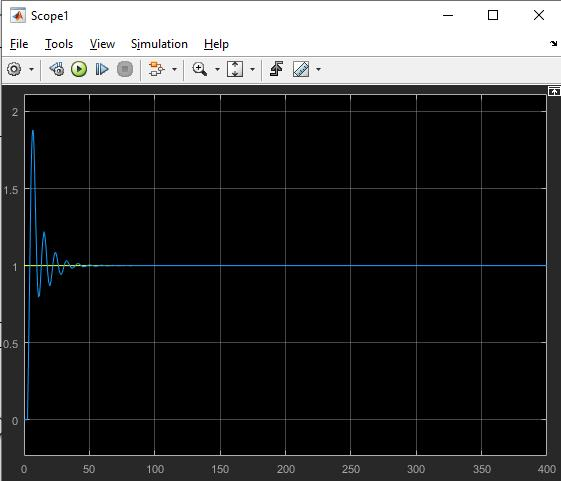
\includegraphics[width=0.8\textwidth]{z1_24}
  \caption{Odziv zatvorenog sistema sa PID regulatorom dobivenim Cohen-Coon metodom}
  \label{fig:z1_24}
\end{figure} 
 
\textbf{8.} U ovom dijelu je potrebno uporediti P, PI i PID regulatore dobivene različitim metodama u stavkama 5., 6. i 7. 

Što se tiče P regulatora, sve tri metode su dale zadovoljavajuće i veoma slične rezultate. 

Što se tiče PI regulatora, najbolji rezultat je dala metoda Ziegler-Nichols koja podrazumijeva dovođenje sistema na granicu stabilnosti. Ovom metodom su dobiveni najkraće vrijeme smirenja, najmanji preskok. Nakon ove metode slijedi Ziegler-Nichols metoda koja podrazumijeva identifikaciju sistema. Ova metoda je dala nešto veće vrijeme smirenja te veći preskok. Najveći preskok je dala COhen-Coon metoda.

Što se tiče PID regulatora, najbolji rezultat je ponovo dala metoda Ziegler-Nichols koja podrazumijeva dovođenje sistema na granicu stabilnosti. Ovom metodom su dobiveni najkraće vrijeme smirenja, najmanji preskok, dok su oscilacije eliminisane. Nakon ove metode slijedi Ziegler-Nichols metoda koja podrazumijeva identifikaciju sistema. Ova metoda je dala veće vrijeme smirenja, veći preskok, a nije eliminisala oscilacije. Najgore rezultate je dala metoda Cohen-Coon koja ima još veći preskok, veće vrijeme smirenja te više oscilacija od Ziegler-Nichols metode koja se zasniva na identifikaciji sistema.

\textbf{9.} Potrebno je vidjeti kako se sistem ponaša kada dodamo smetnju prije upravljanog objekta, tj. simuliramo grešku u aproksimaciji modela sistema. Kao što je navedeno, koriste se parametri iz stavke 5. za sva tri regulatora P, PI i PID. Dobiveni su sljedeći rezultati:

\textbf{P regulator: $K_p=18.36$} (slika \ref{fig:z1_25})

\begin{figure} [H]
  \centering
  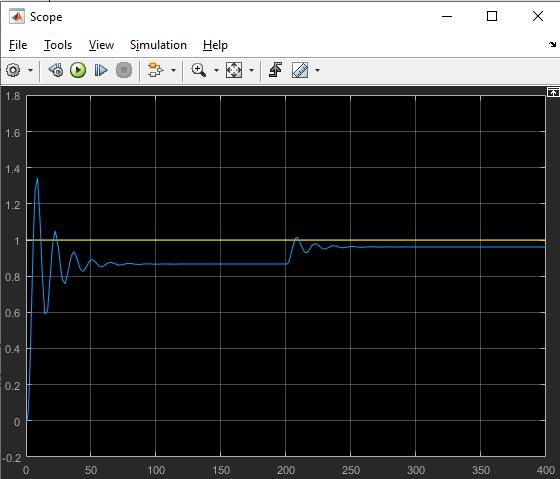
\includegraphics[width=0.75\textwidth]{z1_25}
  \caption{Odziv zatvorenog sistema sa smetnjom sa P regulatorom dobivenim Ziegler-Nichols metodom}
  \label{fig:z1_25}
\end{figure} 

\textbf{PI regulator: $K_p=11.68$, $T_i=14.23$} (slika \ref{fig:z1_26})
 
\begin{figure} [H]
  \centering
  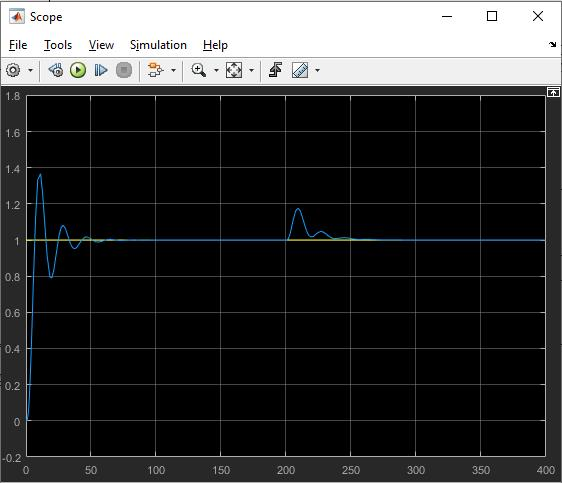
\includegraphics[width=0.75\textwidth]{z1_26}
  \caption{Odziv zatvorenog sistema sa smetnjom sa PI regulatorom dobivenim Ziegler-Nichols metodom}
  \label{fig:z1_26}
\end{figure} 

\textbf{PID regulator: $K_p=20.0292$, $T_i=9.1072$, $T_d=2.2768$} (slika \ref{fig:z1_27})

\begin{figure} [H]
  \centering
  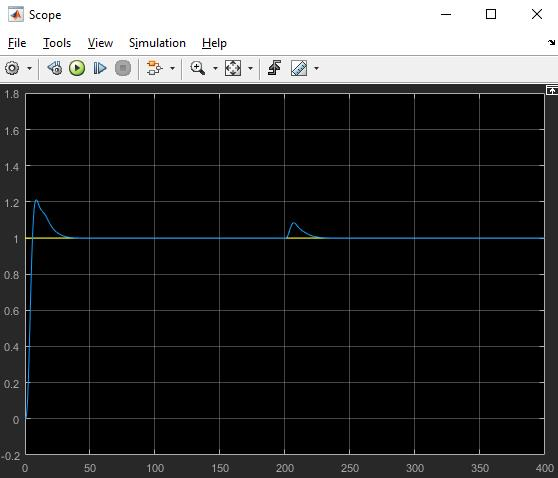
\includegraphics[width=0.8\textwidth]{z1_27}
  \caption{Odziv zatvorenog sistema sa smetnjom sa PID regulatorom dobivenim Ziegler-Nichols metodom}
  \label{fig:z1_27}
\end{figure} 

Step smetnja koja je dodana ispred objekta kojim se upravlja je dodana u trenutku t=200s i njena amplituda je 5. Možemo vidjeti da sam P regulator ne reaguje dobro na dodanu smetnju jer samo pomjeri grešku u stacionarnom stanju na neku drugu vrijednost. PI regulator se dobro nosi sa ovom smetnjom jer I komponenta eliminiše grešku u stacionarnom stanju. PID regulator se također dobro nosi sa ovom smetnjom, jer I komponenta eliminiše grešku u stacionarnom stanju, dok D komponenta smanjuje oscilacije i smanjuje amplitudu preskoka.
















